\chapter{設計}
\label{chap:design}

本章では、本研究において提案する、マイコン向けWebAssembly実行環境の設計を示す。

\section{全体の構成}

本実行環境は、マイコンにおける処理内容をHTTPを用いてインターネット上から取得する。
なお、WebAssemblyは複数モジュールにおける動的リンクにも対応しているが、
本研究では簡便のため単一のモジュールのみを取得し実行するユースケースを想定している。

図\ref{fig:wasm_design}に、本実行環境におけるWebAssemblyプログラムの実行フローを示す。

\begin{figure}[htbp]
  \caption{マイコンにおけるWebAssemblyプログラム実行フロー}
  \label{fig:wasm_design}
  \begin{center}
    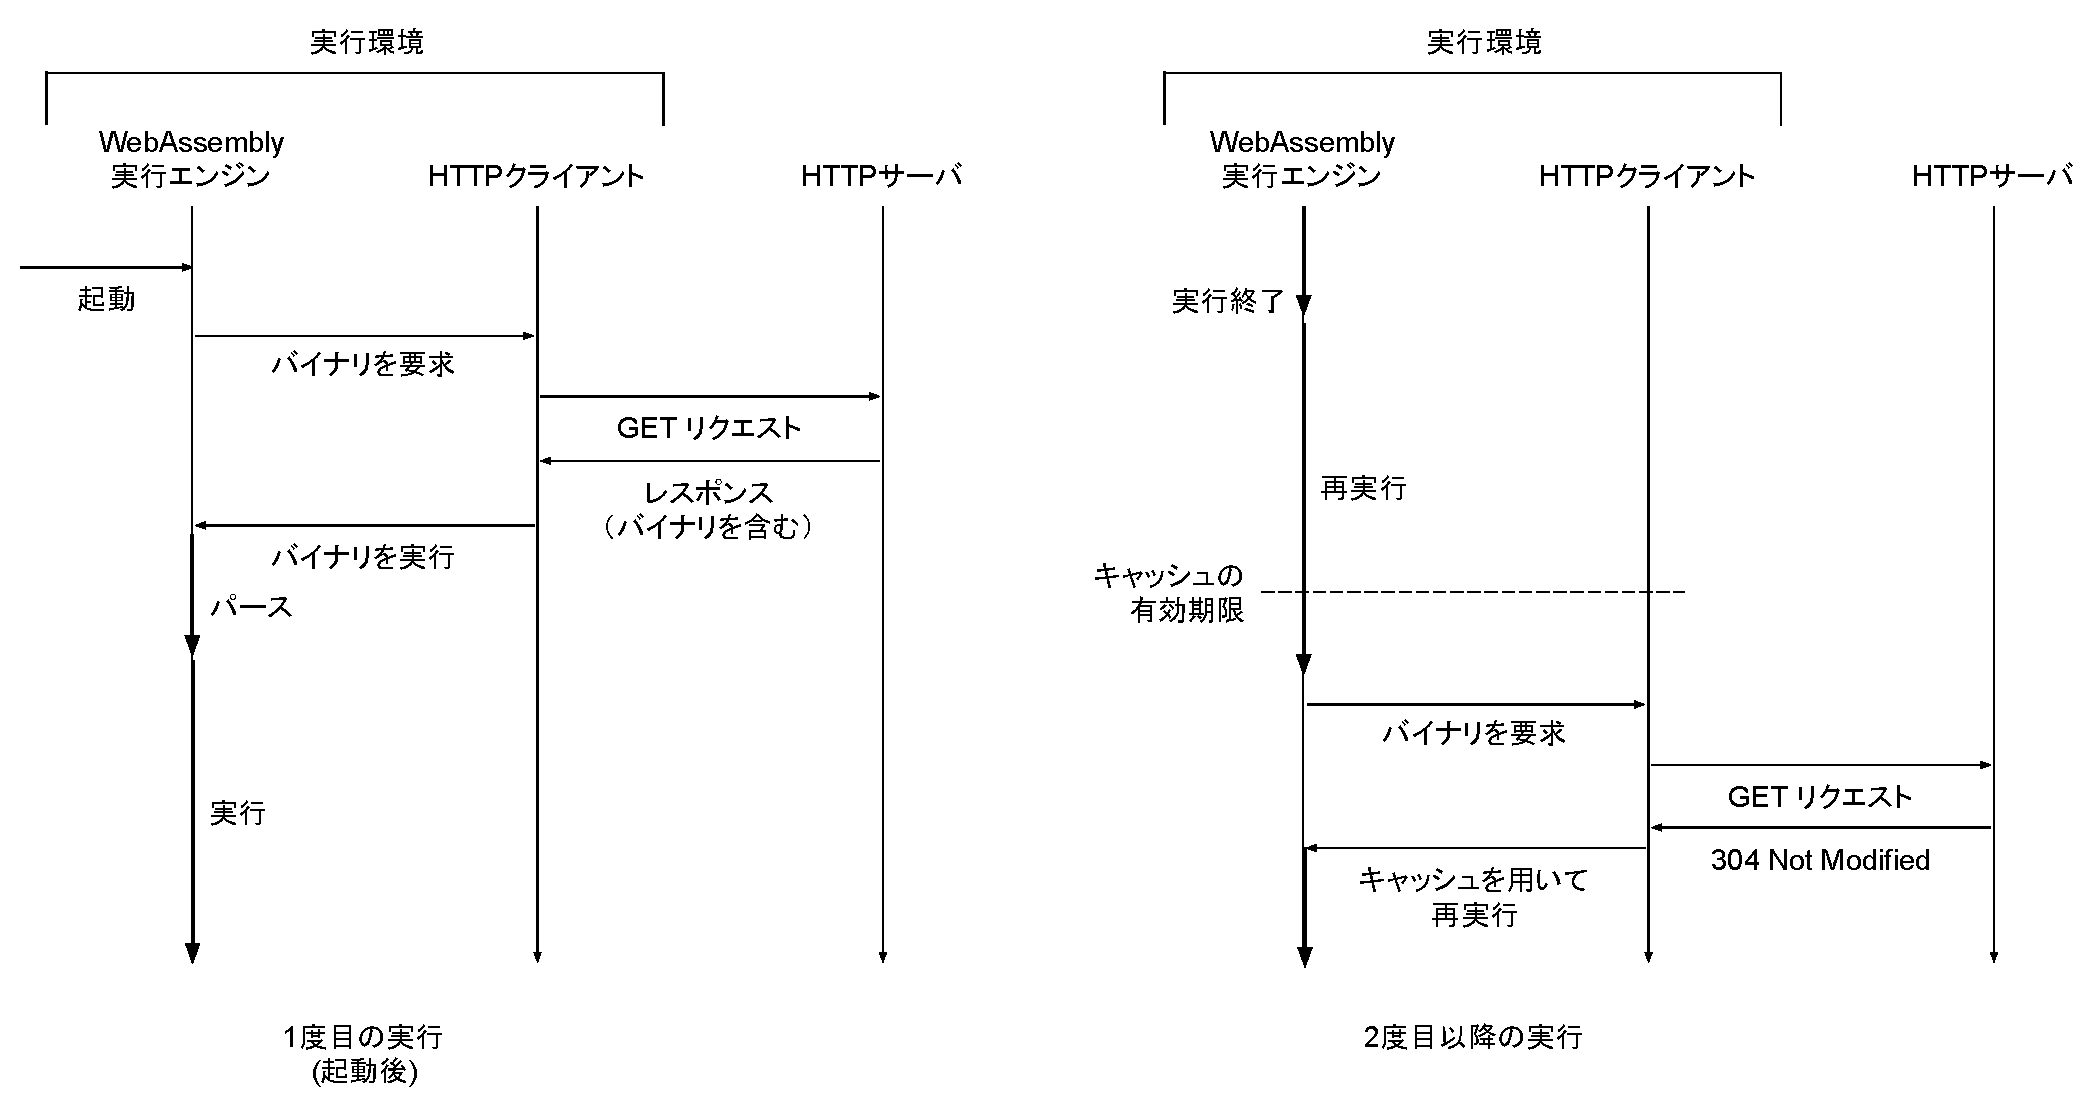
\includegraphics[bb=0 0 1000 530,width=15cm]{img/wasm_design.pdf}
  \end{center}
\end{figure}

\section{WebAssemblyプログラムの取得と実行}

実行環境はマイコンの起動後、ファームウェア書き込み時に指定したURLを用いて、
HTTPサーバからWebAssemblyバイナリを取得する。
実行環境は受け取ったWebAssemblyバイナリをWebAssemblyインタプリタによりパースし、実行する。
実行されるWebAssemblyプログラムは必要に応じて、実行環境を通じてマイコンの入出力にアクセスできる。
WebAssemblyプログラムが実行を終える、または明示的に実行環境へ通知を行うと、
実行環境は現在のWebAssemblyバイナリを破棄し、次に実行するためのWebAssemblyバイナリを
HTTPサーバから再度取得する。

\section{WebAssemblyバイナリ取得の制御}

実行環境は標準的なHTTPユーザーエージェントとして振舞うことで、
特殊なサーバ実装を用意することなく、HTTPレスポンスによりWebAssemblyバイナリ取得の制御を行うことができる。

HTTPサーバからのレスポンスヘッダがキャッシュを許可していれば、
キャッシュが有効な間、実行環境はWebAssemblyバイナリを再取得せずに実行し続ける。
また、実行環境はレスポンスに含まれる\verb|ETag|や\verb|Last-Modified|といった値を保持し、
WebAssemblyバイナリ再取得時のリクエストに含めることで、
バイナリに変更がない場合はレスポンスを\verb|304 Not Modified|ステータスコードのみにできる。
適切にキャッシュを利用することで、通信のための計算負荷、通信帯域を節約できるだけでなく、
WebAssemblyモジュールのパースや初期化を再度行うことなく処理を再開できる。

WebAssemblyバイナリの取得元URLは、HTTPレスポンスステータスコード
\verb|301 Moved Permanently|により恒久的に、
また\verb|302 Found|や\verb|307 Temporary Redirect|により一時的に変更することができる。

また、必要に応じて、Web通信で標準的に用いられる認証や圧縮といった技術を用いて、
通信の安全性や効率を高めることができる。
